\documentclass{article}
\usepackage{graphicx}
\graphicspath{{./images/}}

\title {Data Management SS 2020: Exercise 03, task 3.2}
\date {}

\begin{document}
\maketitle

The sequence I generated was: \\ 7, 14, 2, 5, 1, 13, 6, 16, 9, 11, 19, 15, 18, 3, 10, 20, 4, 8, 12, 17 \\
I inserted the sequence into a B-Tree. I will present a few intermediete steps before the final result. 
Node splitting is first necessary when inserting '1': \\

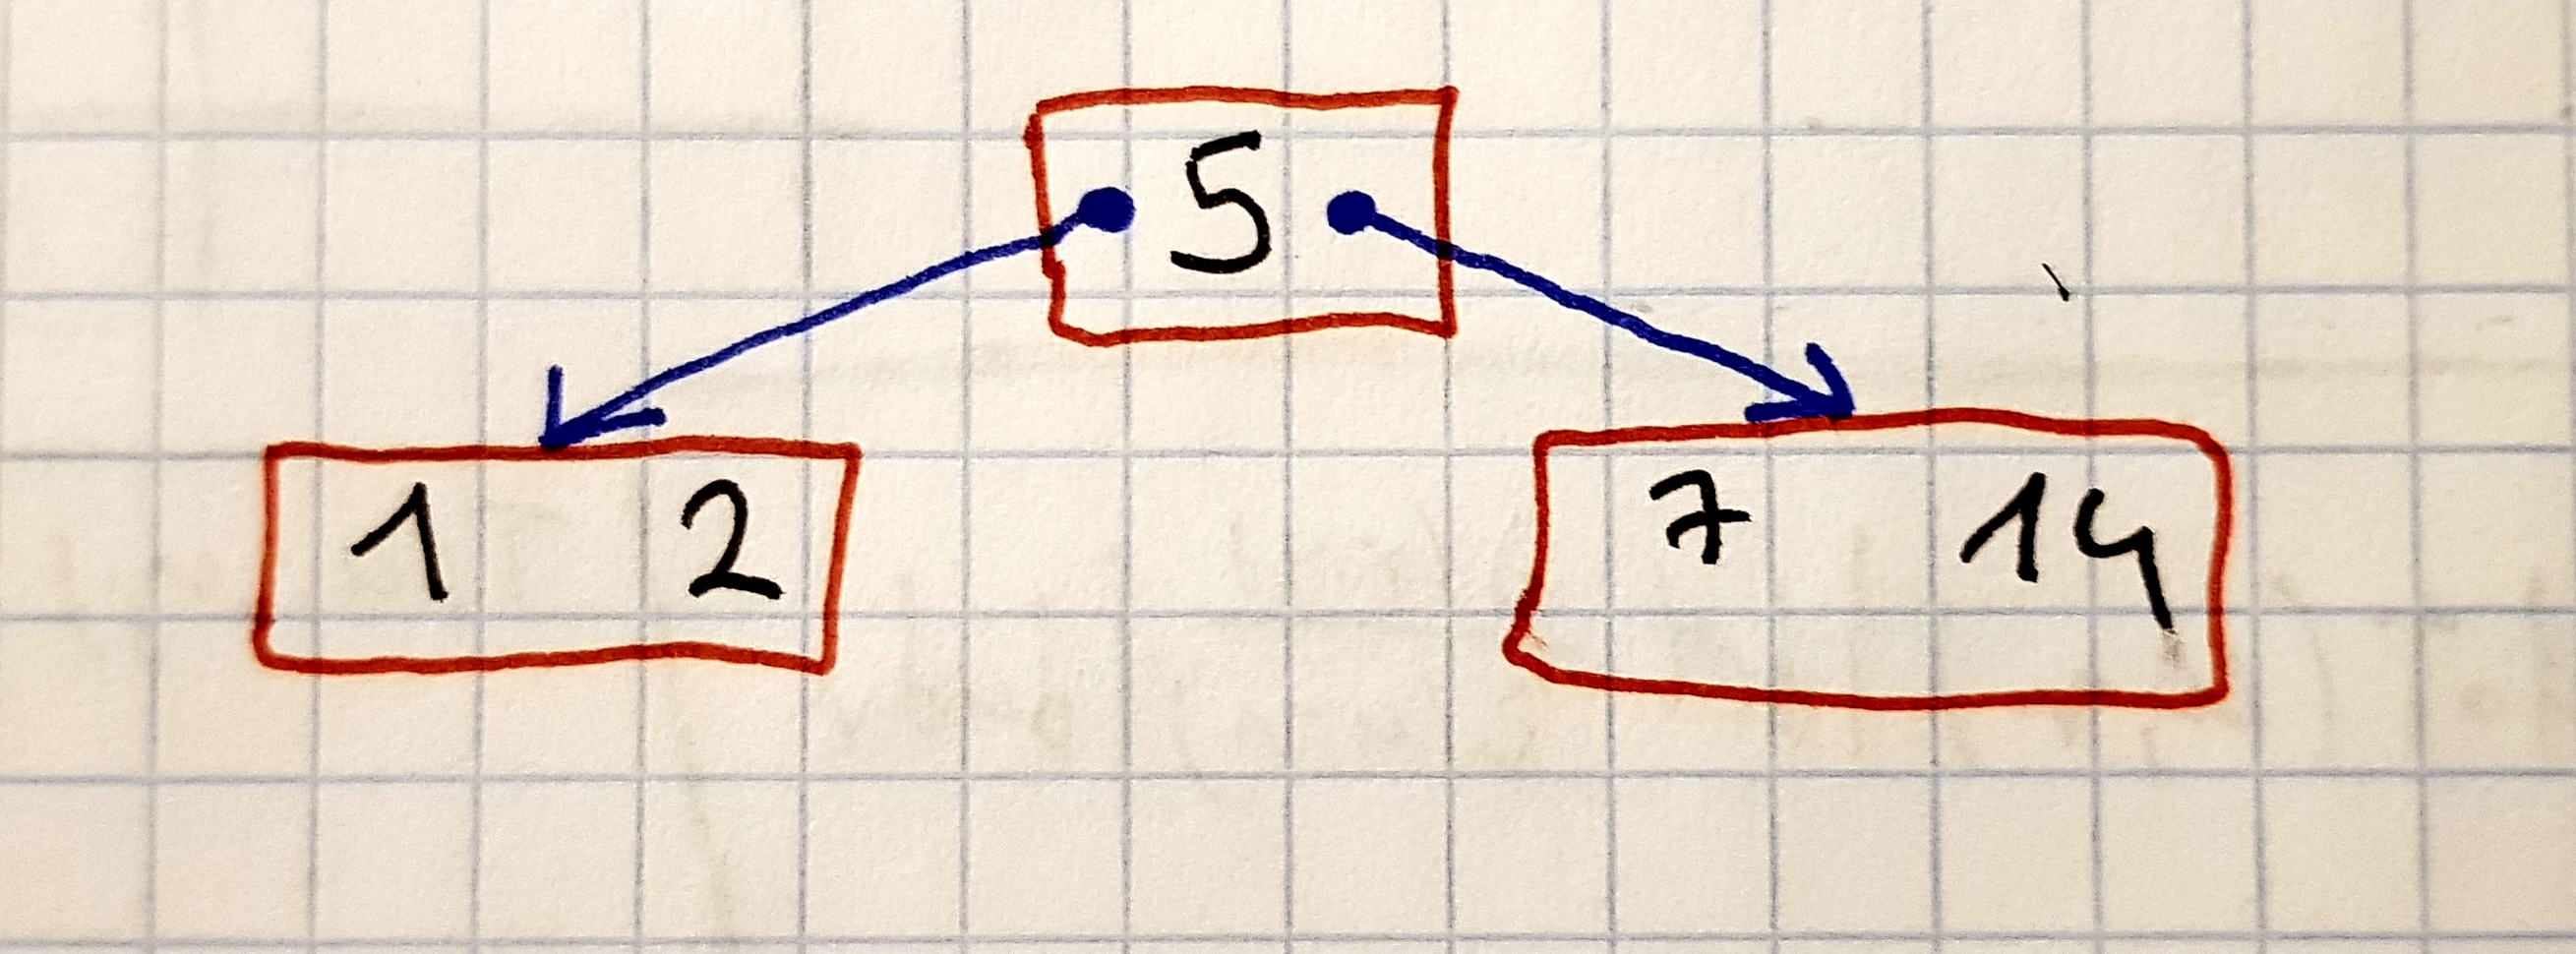
\includegraphics[scale = 0.1]{ins1}
\\ \\
After inserting '16': \\ 
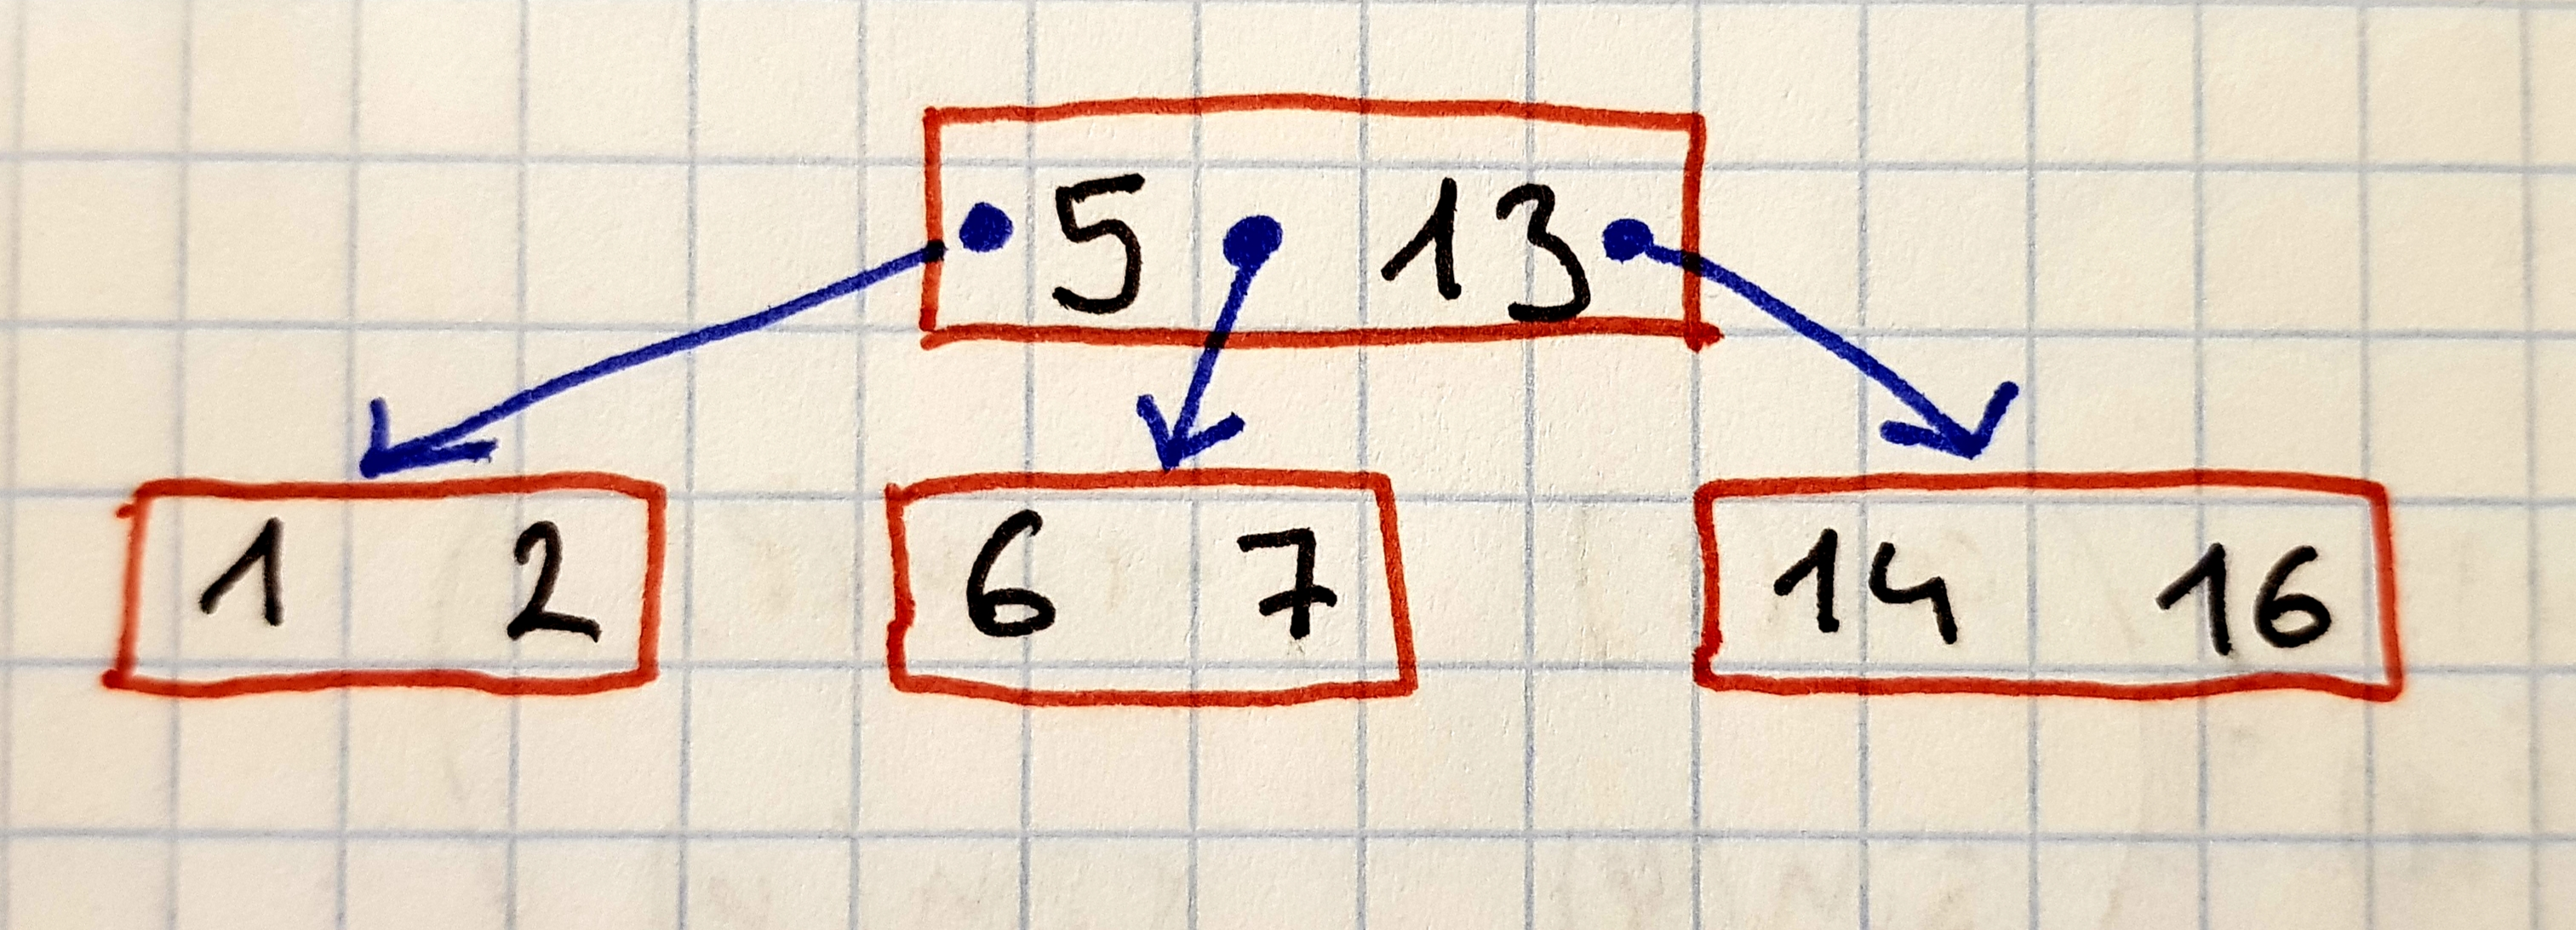
\includegraphics[scale = 0.1]{ins16}
\\ \\
After inserting '18': \\ 
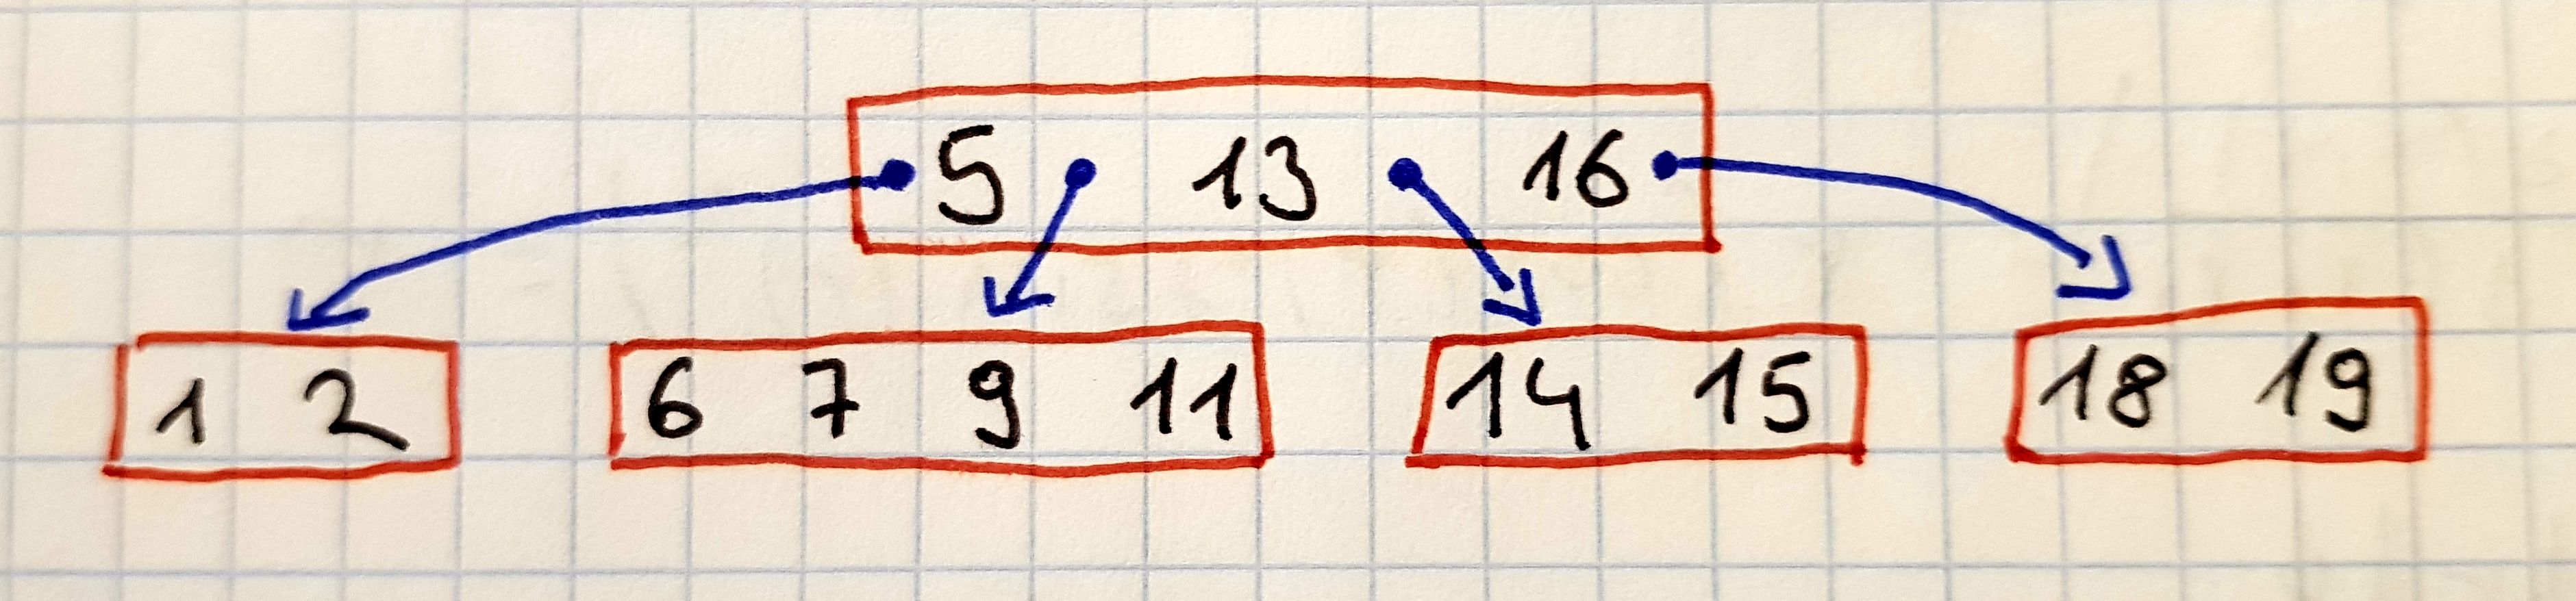
\includegraphics[scale = 0.1]{ins18}
\\ \\ \\ 
After inserting '10': \\ 
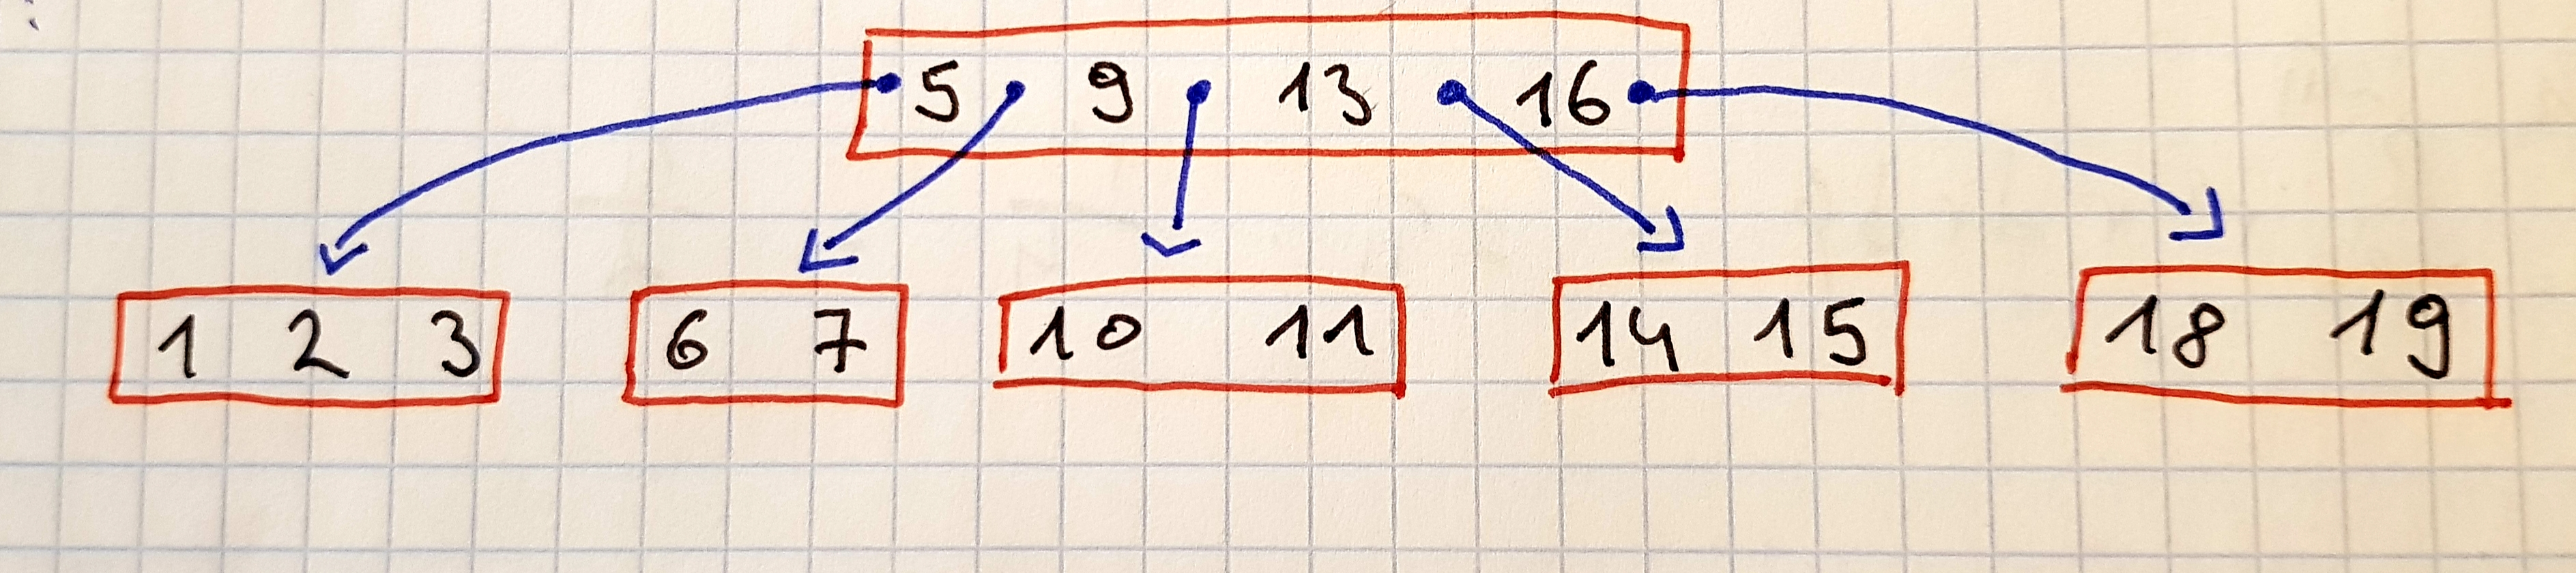
\includegraphics[scale = 0.1]{ins10}
\\ \\
Finally at end we get: \\ 
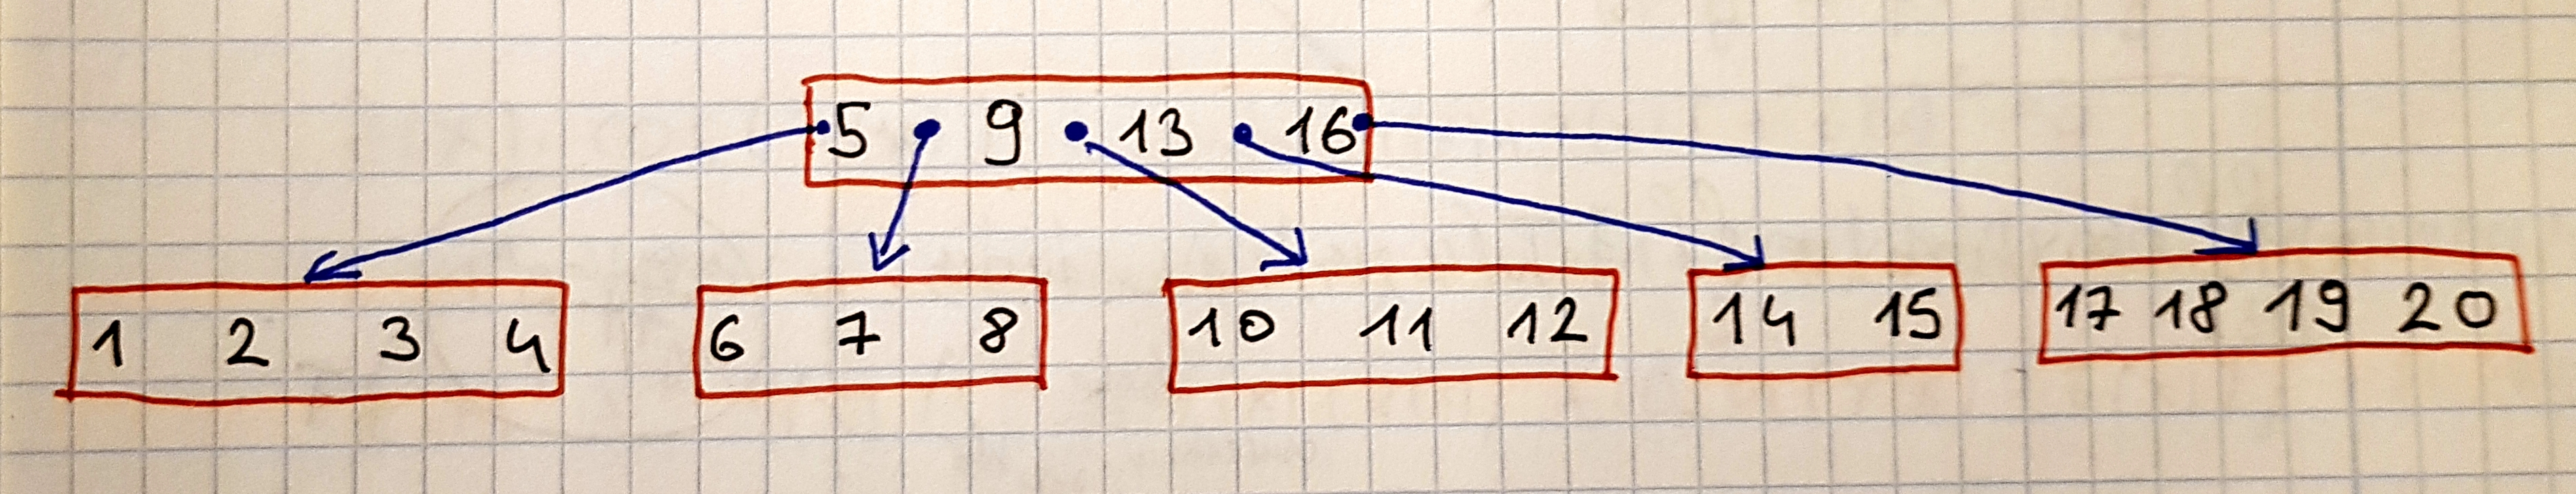
\includegraphics[scale = 0.1]{insfin}
\\ 

For the second part of the task I then removed the keys in the range [8, 14). Here I will also present some intermediate steps: \\
After removing '9': \\ 
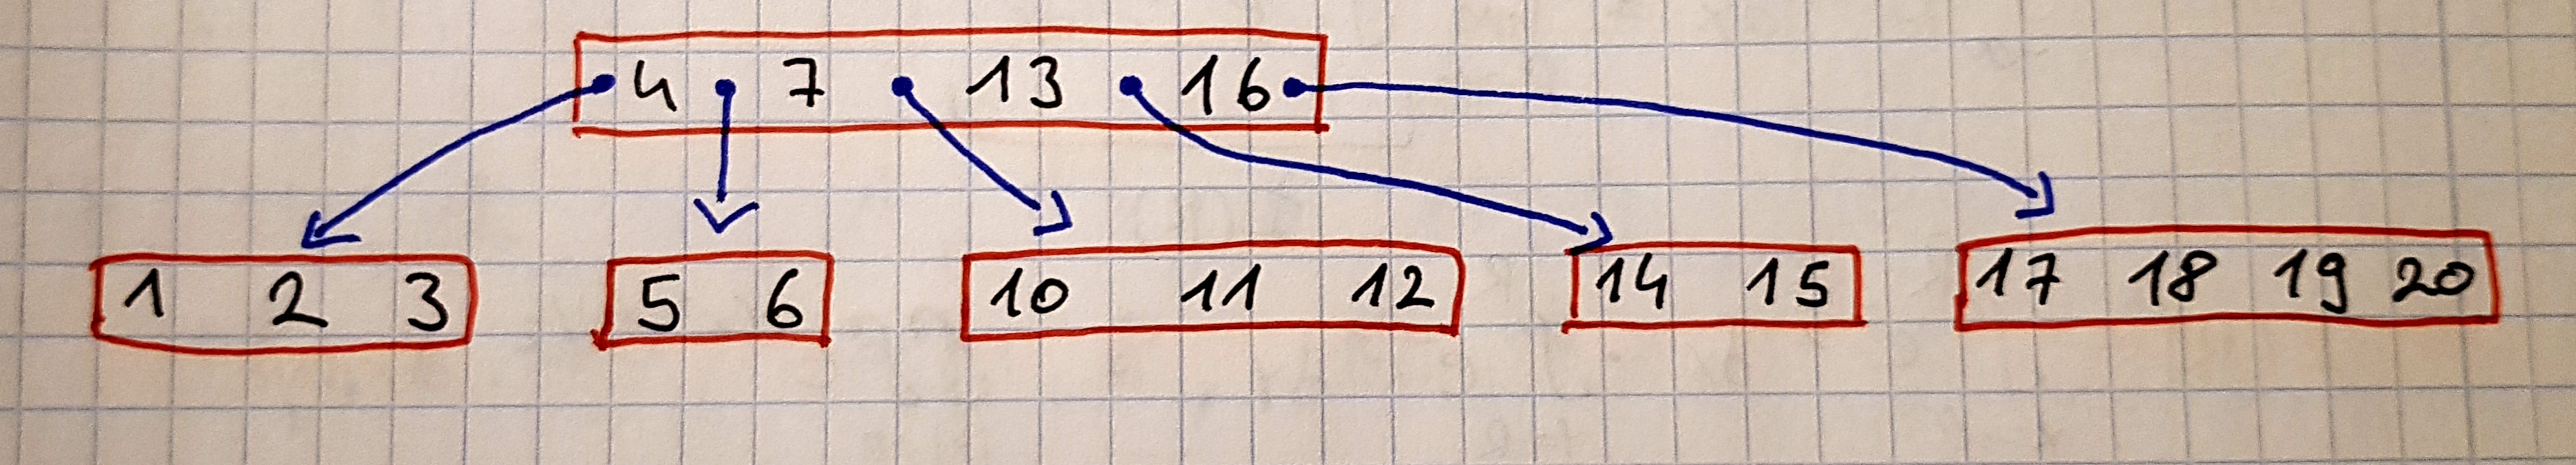
\includegraphics[scale = 0.1]{rem9}
\\ \\
After removing '11': \\ 
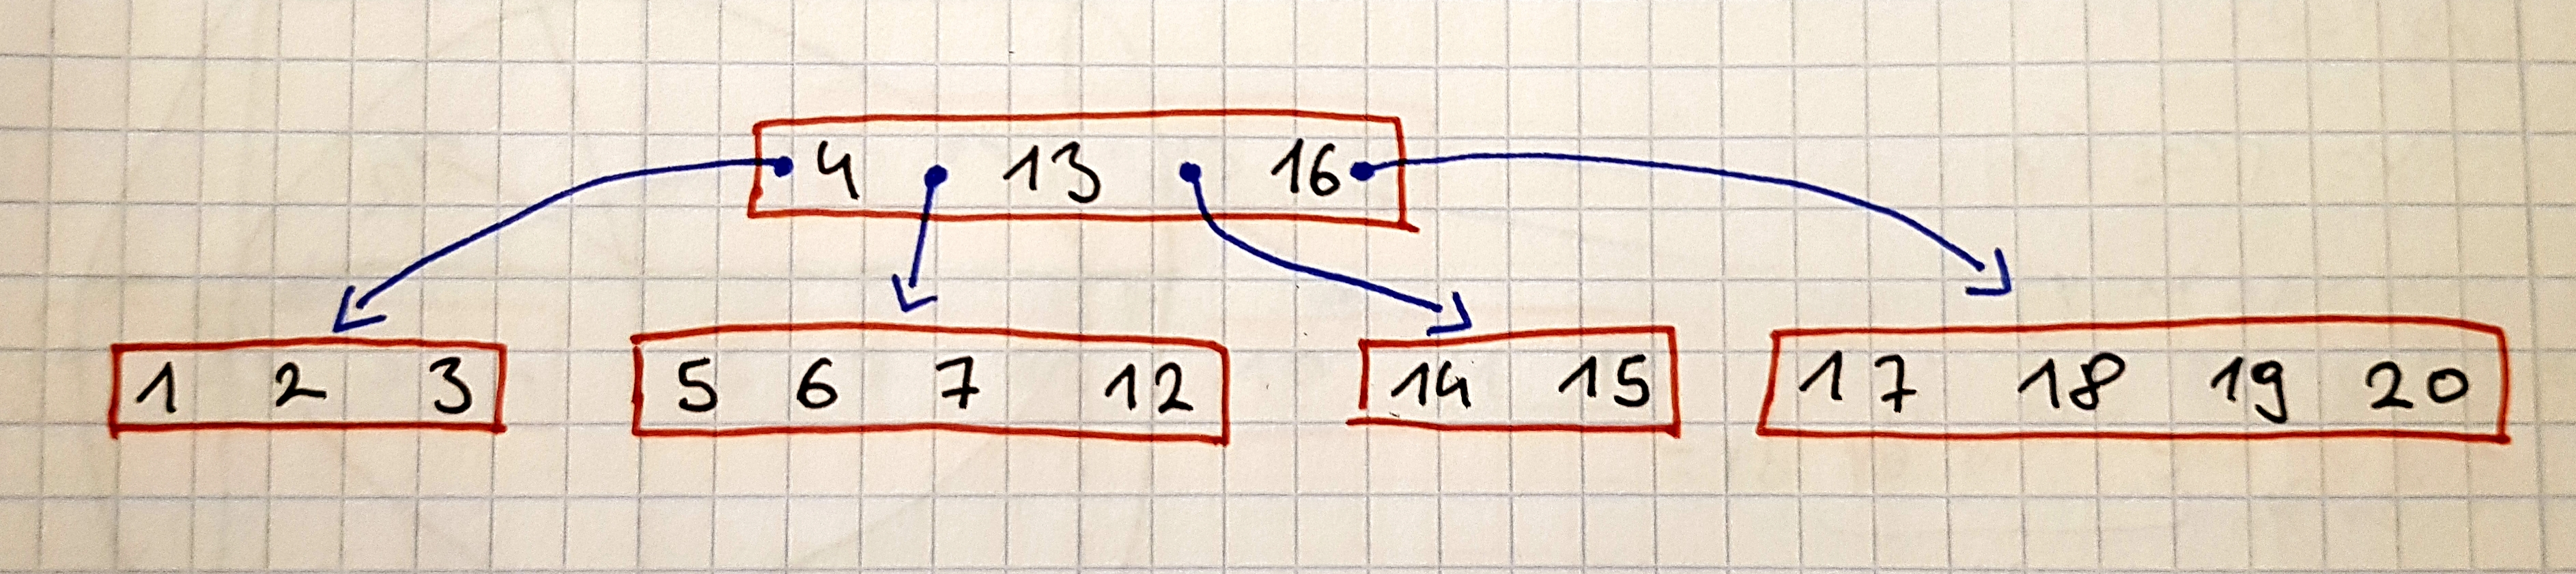
\includegraphics[scale = 0.1]{rem11}
\\ \\
Finally after removing '13': \\ 
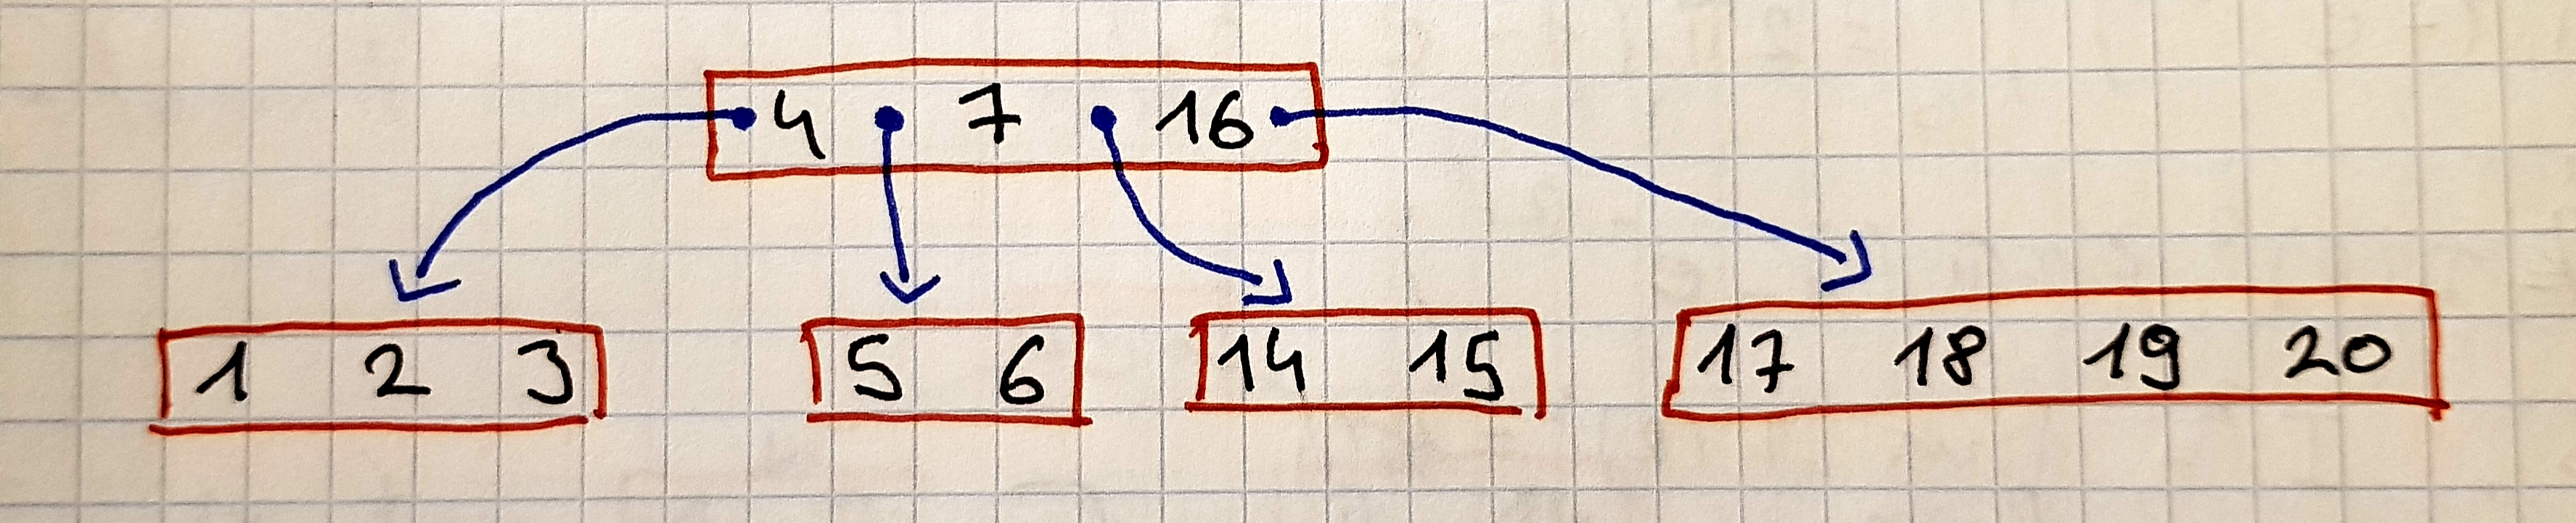
\includegraphics[scale = 0.1]{rem13}
\end{document}